\documentclass[12pt,letterpaper]{article}
\usepackage[utf8]{inputenc}
\usepackage{tikz}
\author{Curso de \LaTeX}
\title{Nodos}
\begin{document}
\maketitle

Un nodo es típicamente un rectángulo, un círculo u otra figura simple con algún texto en su interior. 

Los nodos son una buena herramienta para colocar texto en el interior de una figura.

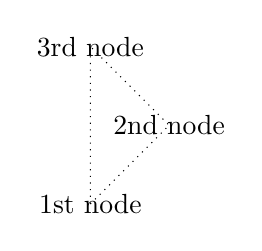
\begin{tikzpicture}
\draw[dotted]
    (0,0) node {1st node}
 -- (1,1) node {2nd node}
 -- (0,2) node {3rd node}
 -- cycle;
\end{tikzpicture}

Podemos definir varias opciones para modificar la apariencia de un nodo:

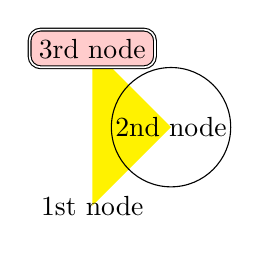
\begin{tikzpicture}
\fill[fill=yellow]
    (0,0) node {1st node}
 -- (1,1) node[circle,inner sep=1pt,draw] {2nd node}
 -- (0,2) node[fill=red!20,draw,double,rounded corners] {3rd node};
\end{tikzpicture}

Para posicionar un nodo en una línea o una curva, utilizamos la opción ``pos''.

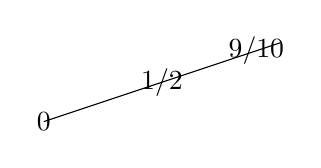
\begin{tikzpicture}
\draw (0,0) -- (3,1)
  node[pos=0]{0} node[pos=0.5]{1/2} node[pos=0.9]{9/10};
\end{tikzpicture}

También podemos colocar un nodo en una posición relativa de una línea o curva, utilizando las opciones de posicionamiento relativo \texttt{left}, \texttt{right}, \texttt{above} y \texttt{below}.

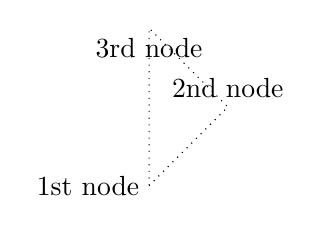
\begin{tikzpicture}
\draw[dotted]
    (0,0) node[left] {1st node}
 -- (1,1) node[above] {2nd node}
 -- (0,2) node[below] {3rd node}
 -- cycle;
\end{tikzpicture}

Finalmente, es posible crear nodos independientes de la líneas, utilizando la instrucción \texttt{\textbackslash node}:

\begin{tikzpicture}
\node[circle, draw] at (0,0) {1er nodo};
\node[circle, draw] at (4,0) {2do nodo};
\node[circle, draw] at (4,4) {3er nodo};
\end{tikzpicture}

Si quisiéramos además enlazar estos nodos, tendríamos que etiquetar cada uno y utilizar la opción \texttt{edge} como se muestra en el ejemplo:

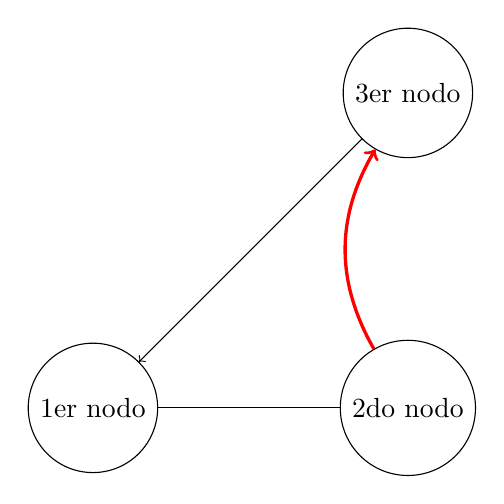
\begin{tikzpicture}
\node[circle, draw] (primero) at (0,0) {1er nodo};
\node[circle, draw] (segundo) at (4,0) {2do nodo}
	edge[-] (primero);
\node[circle, draw] (tercero) at (4,4) {3er nodo}
	edge[very thick,red,bend right,<-] (segundo)
	edge[->] (primero);
\end{tikzpicture}
\end{document}